\section{Humidity}
Atmospheric air includes dry air and water vapor. Recall that for an ideal gas, enthalpy ($h$) is a function of temperature only ($\Delta h = c_p\Delta T$). Notice also from the $h$-$s$ diagram for steam that at relatively low temperatures (<60°C) the water vapor in the air has a constant enthalpy at constant temperature from saturated vapor through the superheated region, thus can be treated as an ideal gas.

From Dalton's Law of Partial Pressures we have for a dry-air/water-vapor mixture that the total pressure $p$ is given by:

\begin{equation}
  p = p_a + p_v
\end{equation}
where subscript $a$ refers to the dry air, and $v$ to the water vapor.
We find it convenient to sketch our processes for the water-vapor component on a $T$-$v$ diagram (which we prefer to the ubiquitous $T$-$s$ diagram in common use, since entropy is not considered in this Section).

\begin{figure}[H]
  \centering
  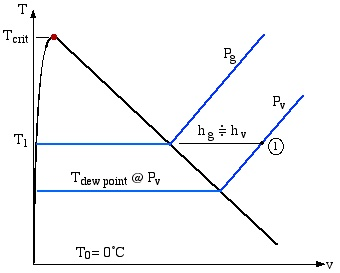
\includegraphics[width=.6\linewidth]{ch7_Tv}
  \caption{A $T$-$v$ diagram illustrating the partial pressure of air and water vapor.}
  \label{fig:ch7_Tv}
\end{figure}

Consider the water vapor shown at state (1) on the diagram. We will find it convenient throughout this section to evaluate enthalpy with respect to $T_0$ = 0°C, since ultimately we only consider differences in enthalpy. From the above diagram:
\begin{equation}
  h_{v@T} = h_{g@T}
\end{equation}
where $g$ refers to the saturated vapor state.
Note that $h_{g@T}$ can be obtained from the saturated vapor tables, or one can use the following shortcut, which has a maximum error of 0.5\% at 60°C:
\begin{equation}
  h_{\rm vapor} = h_{g@T} \approx (2500 + 2 T\ {\rm [°C]})\ [\rm kJ/kg]
\end{equation}

We also evaluate the enthalpy of the dry air component with respect to $T_0$ = 0°C, thus:

\begin{equation}
  h_{\rm dry-air} = c_p T\approx T\ {\rm [°C]}\ [\rm kJ/kg]
\end{equation}

since at the temperatures under consideration, $c_p$ is approximately 1.00 [kJ/kg°C].

In order to evaluate the enthalpy of the atmospheric air we need to first find the mass flow rates of both the dry air and the vapor. We always evaluate these with respect to the mass flow rate of the dry air, and this in turn leads us to the definition of {\bf specific humidity} $\omega$, as follows:

\begin{align}
  \nonumber \dot{m}_a h_{\rm air + vap} &= \dot{m}_a h_a + \dot{m}_v h_v\\
  \nonumber h_{\rm air + vap} &= h_a + \omega h_v\\
  \label{eq:specificHumidity} \omega &= \frac{\dot{m}_{\rm vapor}}{\dot{m}_{\rm dry-air}} = \frac{\dot{m}_{v}}{\dot{m}_{a}}
\end{align}

Note that other terms in common usage are {\bf humidity ratio} or {\bf absolute humidity} to denote specific humidity. The specific humidity can be conveniently determined in terms of the partial pressures $p_a$ and $p_v$ as follows:

\begin{align*}
  \omega &= \frac{\dot{m}_{v}}{\dot{m}_{a}} = \frac{{m}_{v}}{{m}_{a}} = \frac{p_v V / (R_vT)}{p_a V / (R_a T)} = \frac{p_v}{p_a} \frac{R_a}{R_v} =\frac{p_v}{p_a}\frac{0.287\ \rm kJ/kgK}{0.4615\ \rm kJ/kgK}\\
  \omega &= 0.622 \frac{p_v}{p_a} = 0.622 \frac{p_v}{p - p_v}
\end{align*}

Referring to Figure \ref{fig:ch7_Tv}, we now define {\bf relative humidity} $\phi$ as the ratio between the current mass of water vapor and the mass of water vapor in saturated air at the current temperature:
\begin{equation}
  \phi = \frac{m_v}{m_g} =\frac{p_v V / (R_vT)}{p_g V / (R_g T)} = \frac{p_v}{p_g}
\end{equation}

%--------------------------------------------------------------------
\section{The Adiabatic Saturation Process}
%--------------------------------------------------------------------

There is no direct method of measuring specific humidity $\omega$ or relative humidity $\phi$ thus in this section we develop the {\bf adiabatic saturation process}, which leads to the practical {\bf wet \& dry bulb thermometer}, or {\bf sling psychrometer}.

Consider the channel below in which air of unknown humidity enters at station (1) and after absorbing moisture from the liquid pool, exits at 100\% relative humidity at station (2). This process is also shown on the $T$-$v$ diagram below.



